\documentclass[dvipdfmx,autodetect-engine,titlepage]{jsarticle}
\usepackage[dvipdfm]{graphicx}
\usepackage{ascmac}
\usepackage{fancybox}
\usepackage{listings}
\usepackage{plistings}
\usepackage{itembkbx}
\usepackage{amsmath}
\usepackage{url}
\usepackage{graphics}
\usepackage{here}

\lstset{
  basicstyle={\ttfamily},
  identifierstyle={\small},
  commentstyle={\smallitshape},
  keywordstyle={\small\bfseries},
  ndkeywordstyle={\small},
  stringstyle={\small\ttfamily},
  frame={tb},
  breaklines=true,
  columns=[l]{fullflexible},
  numbers=left,
  xrightmargin=0zw,
  xleftmargin=3zw,
  numberstyle={\scriptsize},
  stepnumber=1,
  numbersep=1zw,
  lineskip=-0.5ex
}

\textheight=23cm
\renewcommand{\figurename}{図}
\renewcommand{\tablename}{表}
\newenvironment{code}
{\vspace{0.5zw}\VerbatimEnvironment  \begin{screen} 
\baselineskip=1.0\normalbaselineskip
 \begin{Verbatim}}
{\end{Verbatim}
\baselineskip=\normalbaselineskip
 \end{screen}\vspace{0.5zw}} 

\title{ワイヤレス通信システム(B1)\\
8th Week 半値角\\
}
\author{2600200087-2\\Oku Wakana\\奥 若菜}
\date{Jun. 19 2022}

\begin{document}

\maketitle

\section{半値角}
\subsection{問題}
教科書36ページの式(3.37)を計算し、半値角が78度となることを数値的に検証せよ。\\

\subsection{検証過程}
下の図1は、0から2πにおいて、式(3.37)より、指向性係数を表したグラフである。図1より、Dが最大となるのは\begin{math}
  \theta = 1/2 \pi
\end{math}
のときだと分かる。また、0から\begin{math}
\pi
\end{math}
の範囲で、Dは\begin{math}\theta = 1/2 \pi\end{math}を軸に対称な値をとることから、半値角も同様に、
\begin{math}\theta = 1/2 \pi\end{math}を中心に78度の範囲をとる。すなわち\begin{math}\theta = 1/2 \pi\end{math}を中心に左右に39度ずつ範囲をとることになる。
半値角は電界強度が最大放射方向から1/√2に低下する範囲である。よって、半値角が78度ならば、1/πから39度ずつ角度を増減させた角度において、指向性係数Dの値は、1/√
2となるはずである。\\

\begin{figure}[H]
  \centering
  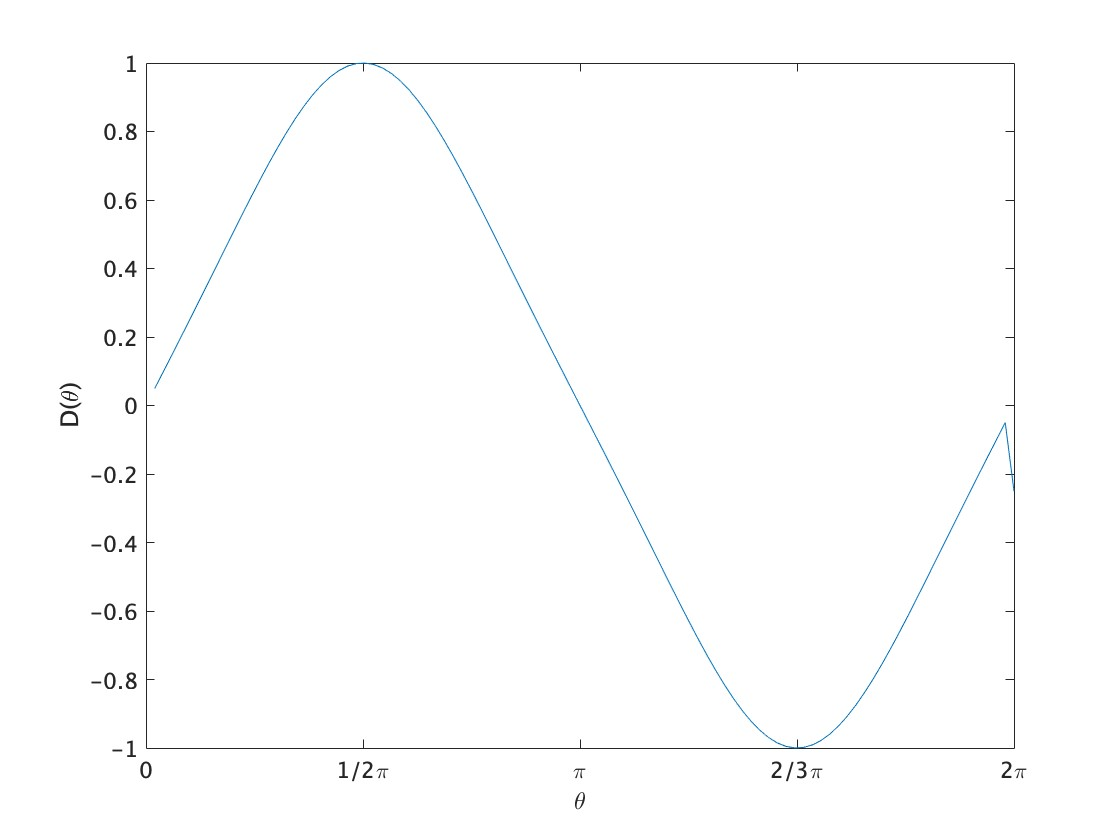
\includegraphics[scale=0.28]{f1.jpg} 
  \caption{完全半波長アンテナの指向性係数}\label{fig:図1}
\end{figure}

図2は、1/πから39度ずつ角度を増減させた角度と、D=1/√2となる位置に破線をひいたものである。グラフから、半値角が78度の範囲が、ちょうどD=1/√2の境界になっていることが分かる。よって、半値角が78度となることが検証できた。

\begin{figure}[H]
  \centering
  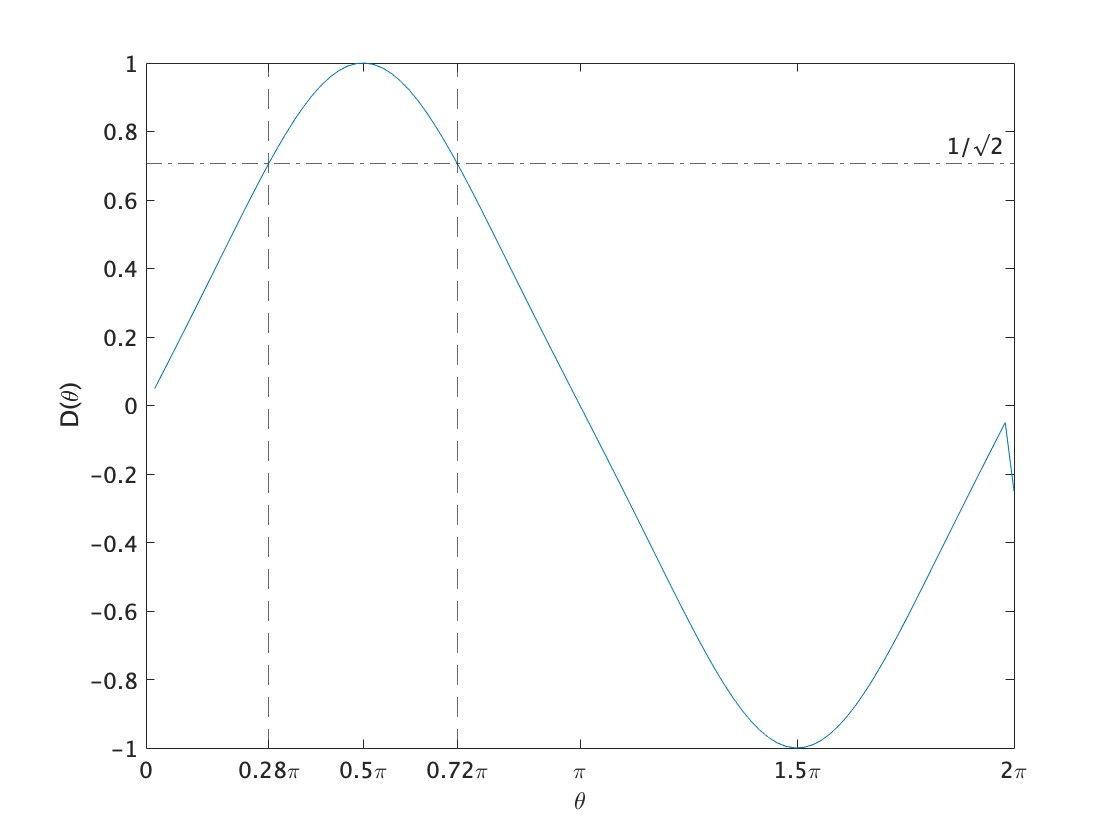
\includegraphics[scale=0.28]{week8.jpg} 
  \caption{完全半波長アンテナの指向性係数}\label{fig:図2}
\end{figure}

下に、グラフ作成の際に使用したMATLABのソースコードを示す。\\


\begin{lstlisting}[caption=ソースコード,label=1]
  figure

%Pは円周率
P = pi;

%x軸を0から2の範囲に設定する
S = linspace(0,2);

%θに対する指向性係数Dを求める
D = cos( P/2 .* cos(S .* P))./sin(S .* P);

%グラフを描画
plot(S,D)

%Dが最大となる0.5πから、半値角78度の半分の39度を足し引きした角度を求める
A = 0.5 - (39 / 180);
B = 0.5 + (39 / 180);

%半値角での指向性係数Dを求め、表示する
halfA = cos( P/2 * cos(A * P)) / sin(A * P);
halfB = cos( P/2 * cos(B * P)) / sin(B * P);
sprintf('halfA: %f',halfA)
sprintf('halfB: %f',halfB)

%見やすいように目盛りを設定
xticks([0 A 0.5 B 1 1.5 2])
xticklabels({'0',string(round(A,2))+'\pi','0.5\pi',string(round(B,2))+'\pi','\pi','1.5\pi','2\pi'})

%半値角78度がDの最大値の1/√2になるか確認
xline([A,B],'--')
yline(1/sqrt(2),'-.','1/\surd2')

%ラベル設定
xlabel('\theta')
ylabel('D(\theta)')
  
\end{lstlisting}

\subsection{評論}
「微小ダイポールアンテナは小型であるがこれを半波長にまで大きくしてもその指向性の絞られ具合は90度から78度とほとんど変わらない、この意味で微小ダイポールアンテナは大きさを考え実用的である」という意見
について述べる。\\

検証の結果、実際に指向性が78度に絞られることが確認できた。90度から78度に指向性を絞ることで、大きな利益が得られないのであれば、低周波で半波長アンテナを設計するなどすると、アンテナが非常に大きくなり実用的ではないため、微小ダイポールアンテナは大きさを考え実用的であるという意見は正しいと言える。
\end{document}
